% Created 2016-11-04 Fri 13:47
\documentclass[11pt]{article}
\usepackage[utf8]{inputenc}
\usepackage[T1]{fontenc}
\usepackage{fixltx2e}
\usepackage{graphicx}
\usepackage{longtable}
\usepackage{float}
\usepackage{wrapfig}
\usepackage{rotating}
\usepackage[normalem]{ulem}
\usepackage{amsmath}
\usepackage{textcomp}
\usepackage{marvosym}
\usepackage{wasysym}
\usepackage{amssymb}
\usepackage{hyperref}
\tolerance=1000
\usepackage{graphicx}
\author{Young}
\date{\today}
\title{STEM}
\hypersetup{
  pdfkeywords={},
  pdfsubject={},
  pdfcreator={Emacs 24.5.1 (Org mode 8.2.10)}}
\begin{document}

\maketitle

\section{Linear Regression}
\label{sec-1}
\subsection{{\bfseries\sffamily DONE} Simple Linear Regression 10/15/16}
\label{sec-1-1}
\[I.mult = \beta_1*(I.conv)+\beta_0\]
For the initial model, I reduced the two data sets from 3D to 1D and
performed linear regression with a bias term. The least squares
estimates for intercept is 0 and slope is 0.0011319. 

It is clear that relationship between the two image sets is not linear
(see scatter plot with regression line). Also, there seems to be
descrete "jumps" in the response variable that the linear model does
not capture. I did not try cross-validation with the initial model.

There are many ways to improve the model. First, I would build a model
that imposes a restriction on the response variable. One example would
be logistic transformation which will output in the range of [0,1]. We
could then rescale the output to match the range of the Multislice
image intensities.  

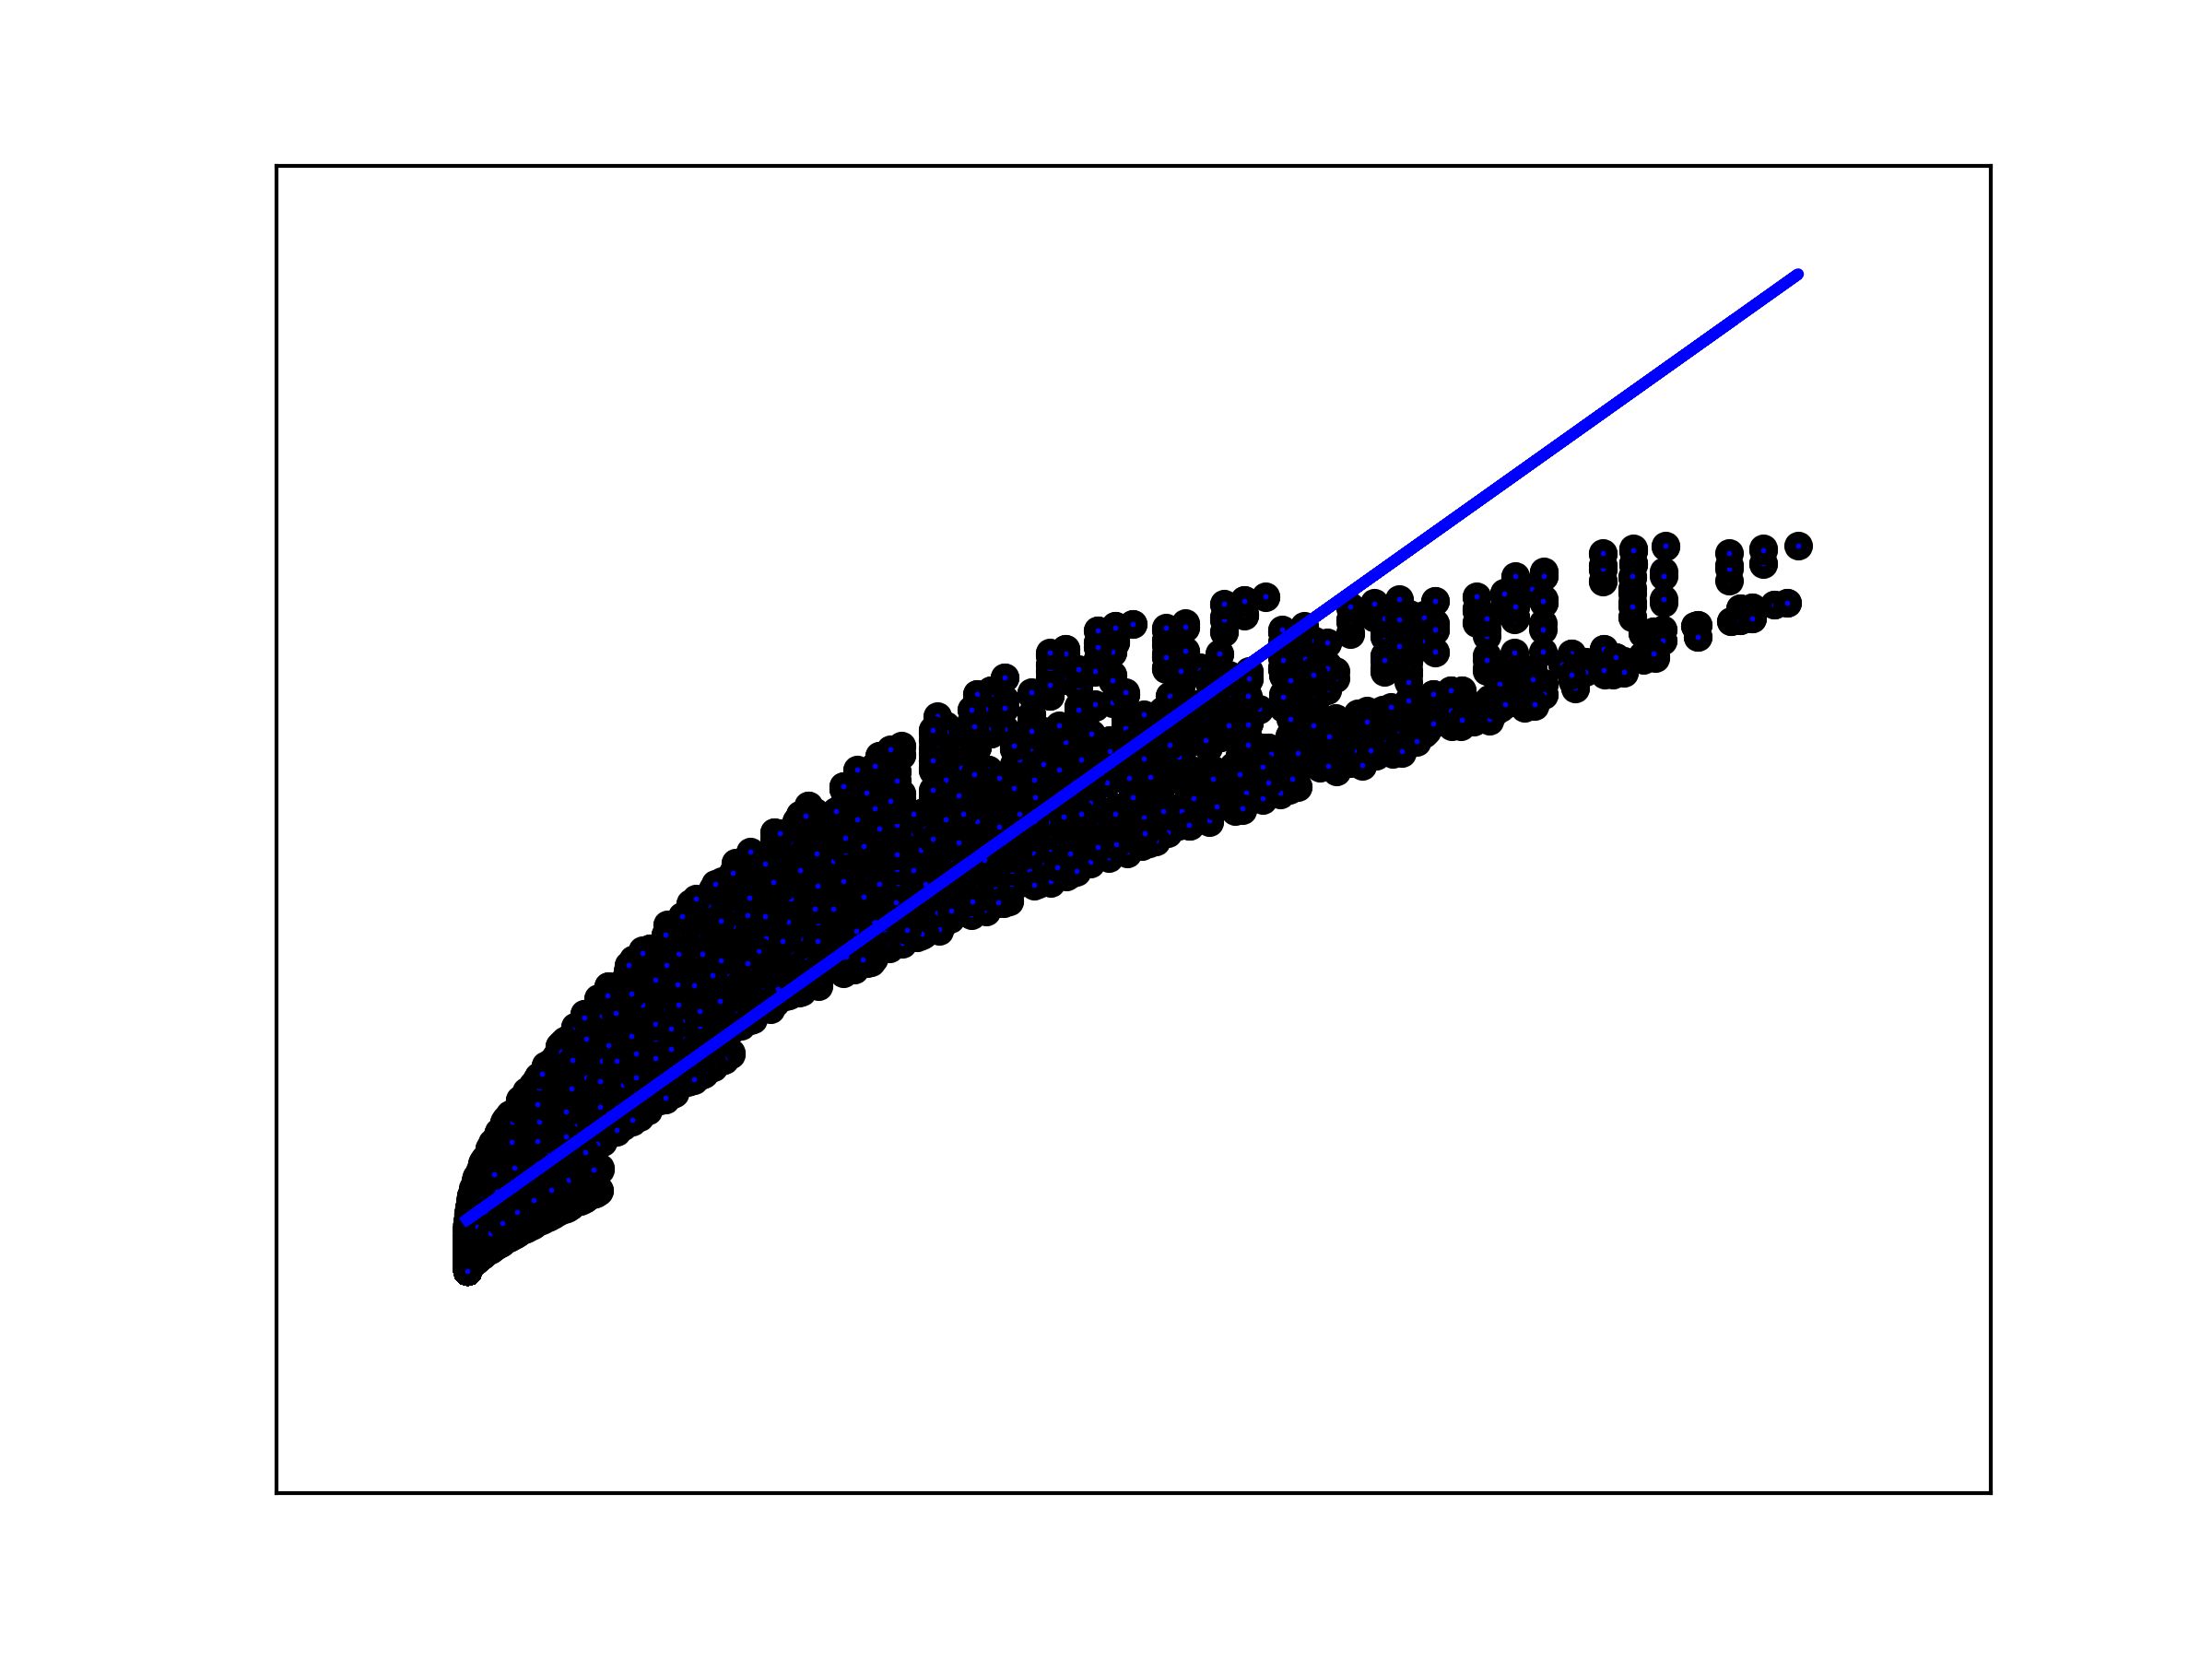
\includegraphics[width=.9\linewidth]{./images/slr.png}

Secondly, I would develop a feature set that has more explantory
power. One natural way to start would be to include the dimensional
indices as features to account for spatial correlation. However, this
could be complicated as there seems to be clusters of high intensity
pixels in the center and corners of the image. Either a kernel method
or K-means method might be useful to account for spatially-clustered
pixel intensities. Alternatively, we could perform segmentation on the
different regions.

Third, some form of piecewise model (i.e. Decision Trees) or
locally-weighted models might better account for "jumps".

\begin{itemize}
\item Python files: olr.py
\end{itemize}
\pagebreak
\subsection{Multiple Regression 10/30/16}
\label{sec-1-2}
For each layer, I generated a .png file with side by side images of
convolution, multislice, and their difference (after
normalization). These files are in data/images/ directory.  It looks
like multislice images tend to be smoother than convolution images.

I fit various multiple linear regression models using

\begin{itemize}
\item 1 pixel or 9 pixels (pixel and 8 neighbors)
\item gradient direction/magnitude
\item linear and quadratic predictors
\end{itemize}

The graphs below show the predicted outcome vs. observed (multiscale)
intensity as a measure of model fit. It's clear that adding the
quadratic term improves the model fit significantly. Gradient
information doesn't seem to improve the model beyond the quadratic
terms of the neighbor intensities. 

I plan to perform cross-validation to compare these models. I also
would like to experiment with applying smoothing filters to the
convolution image. 
\pagebreak

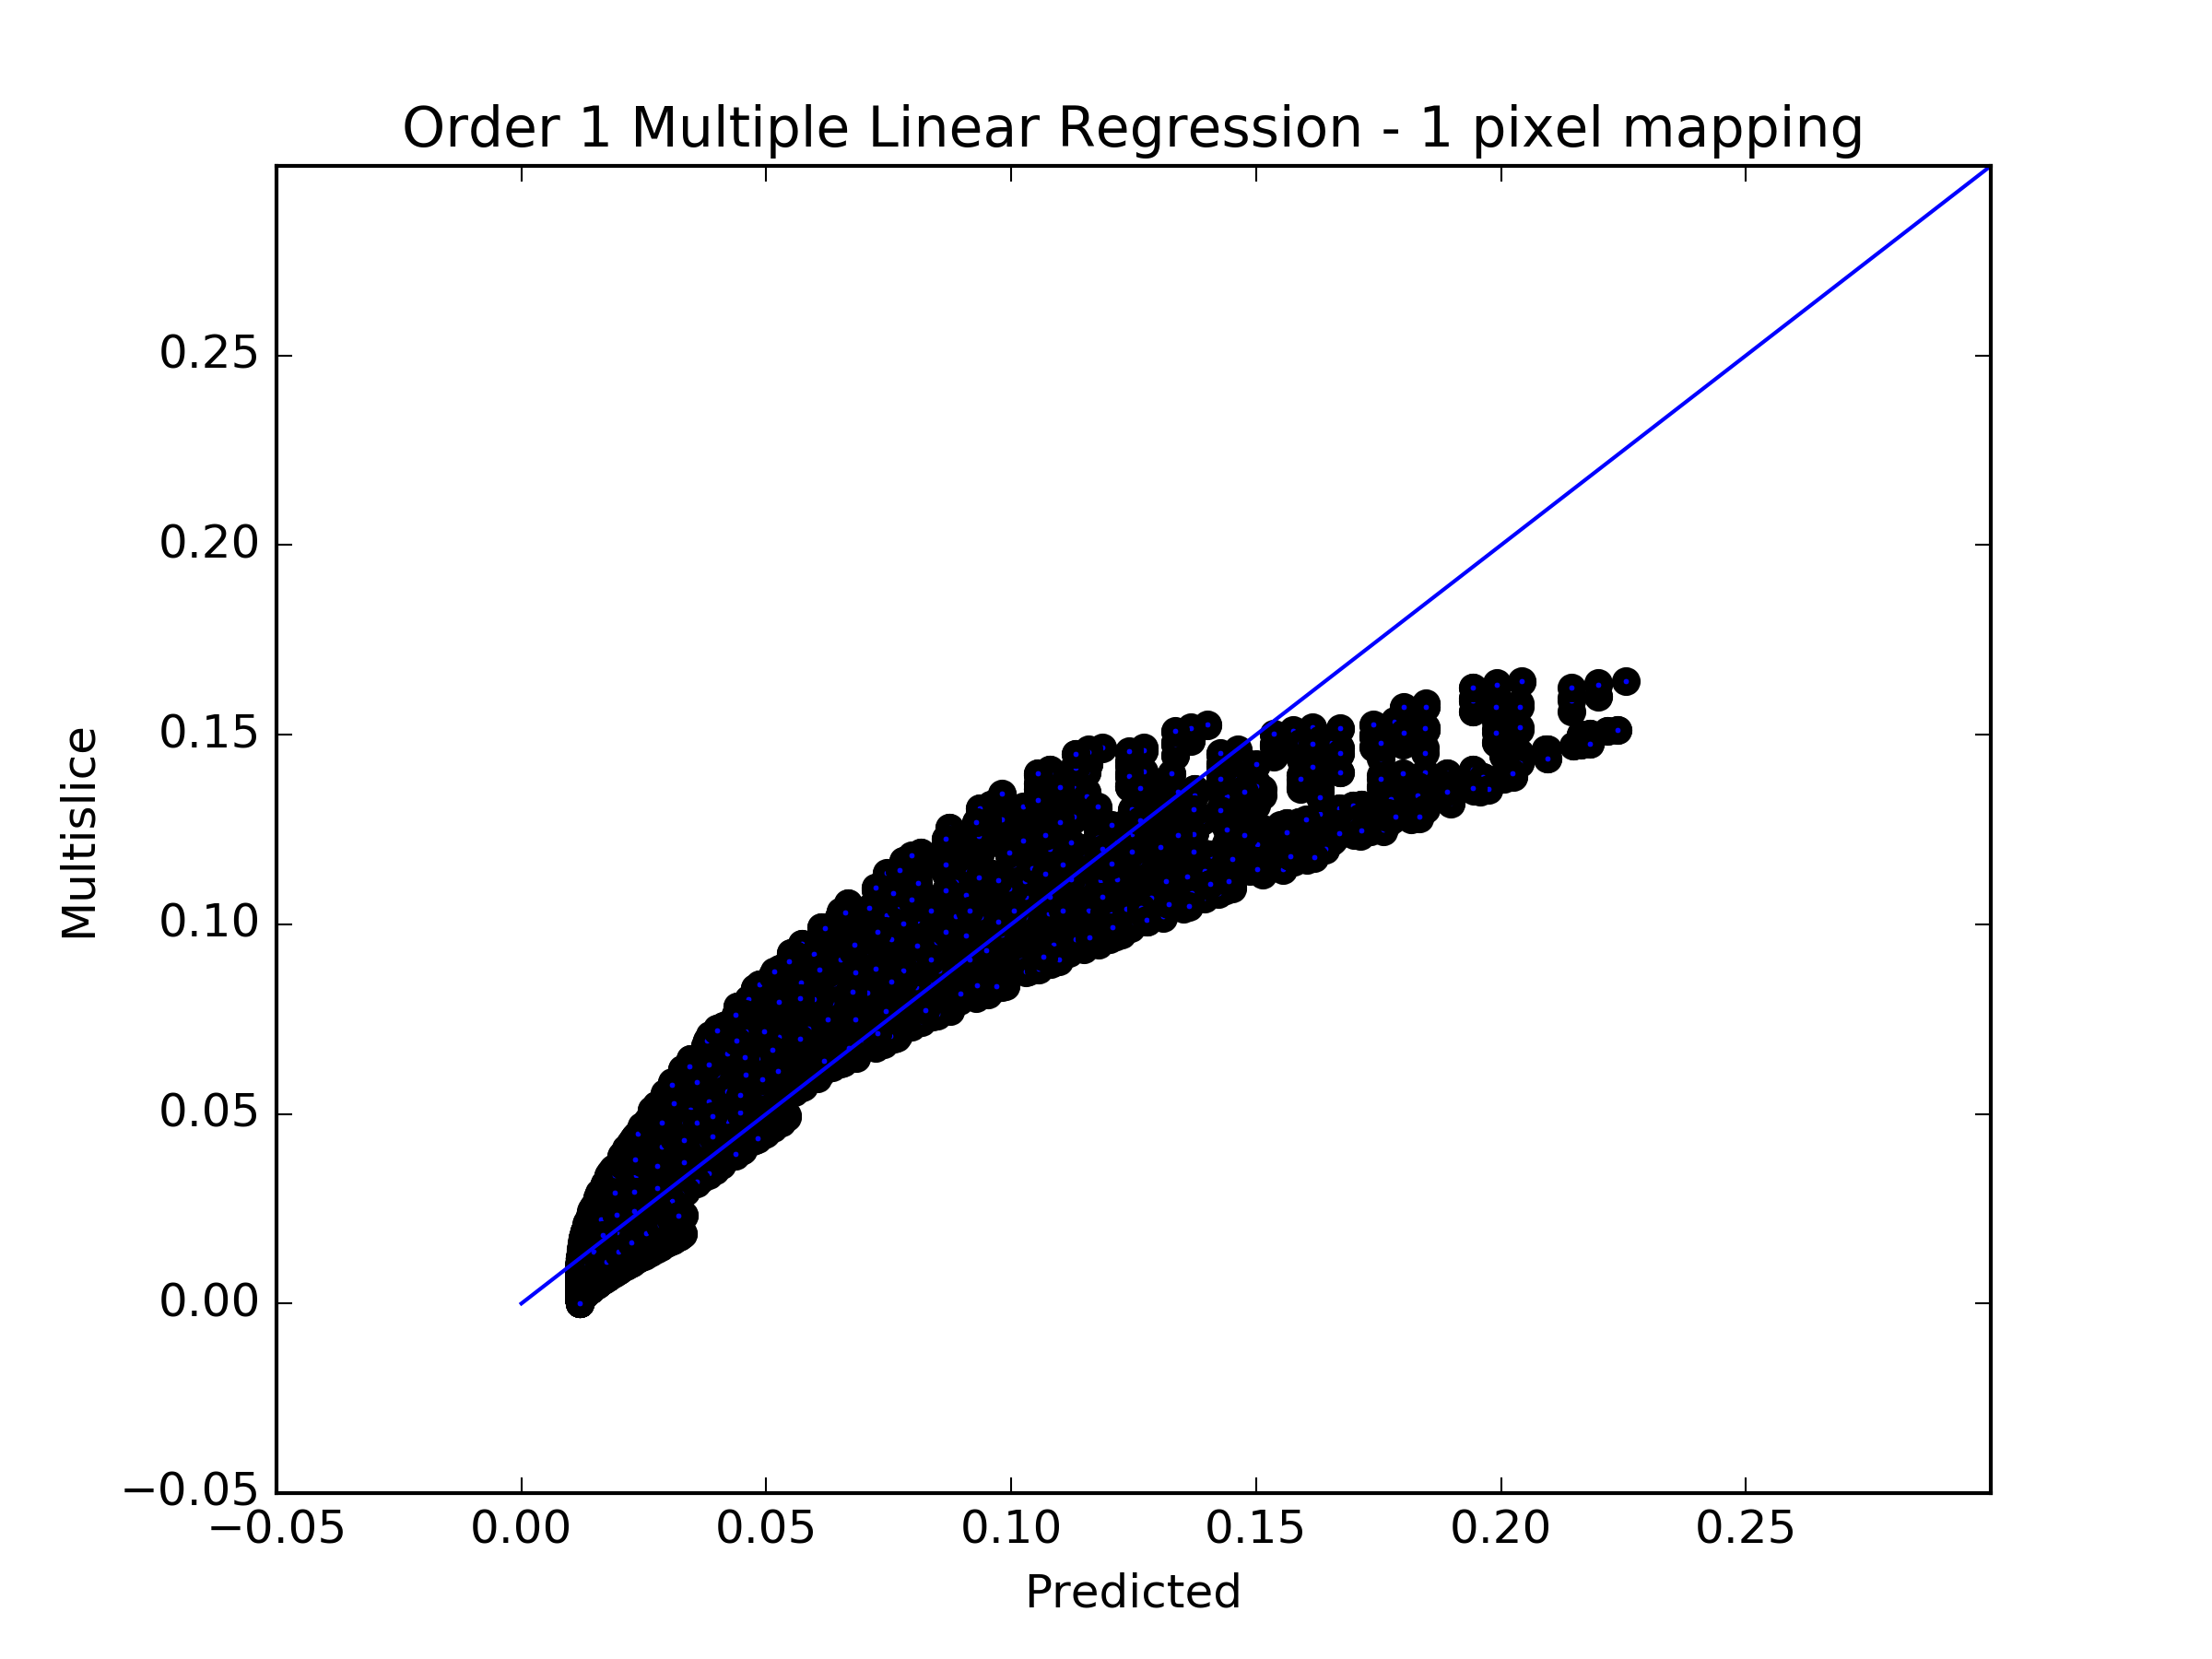
\includegraphics[width=.9\linewidth]{./images/olr_order1_1pixel.png}\\
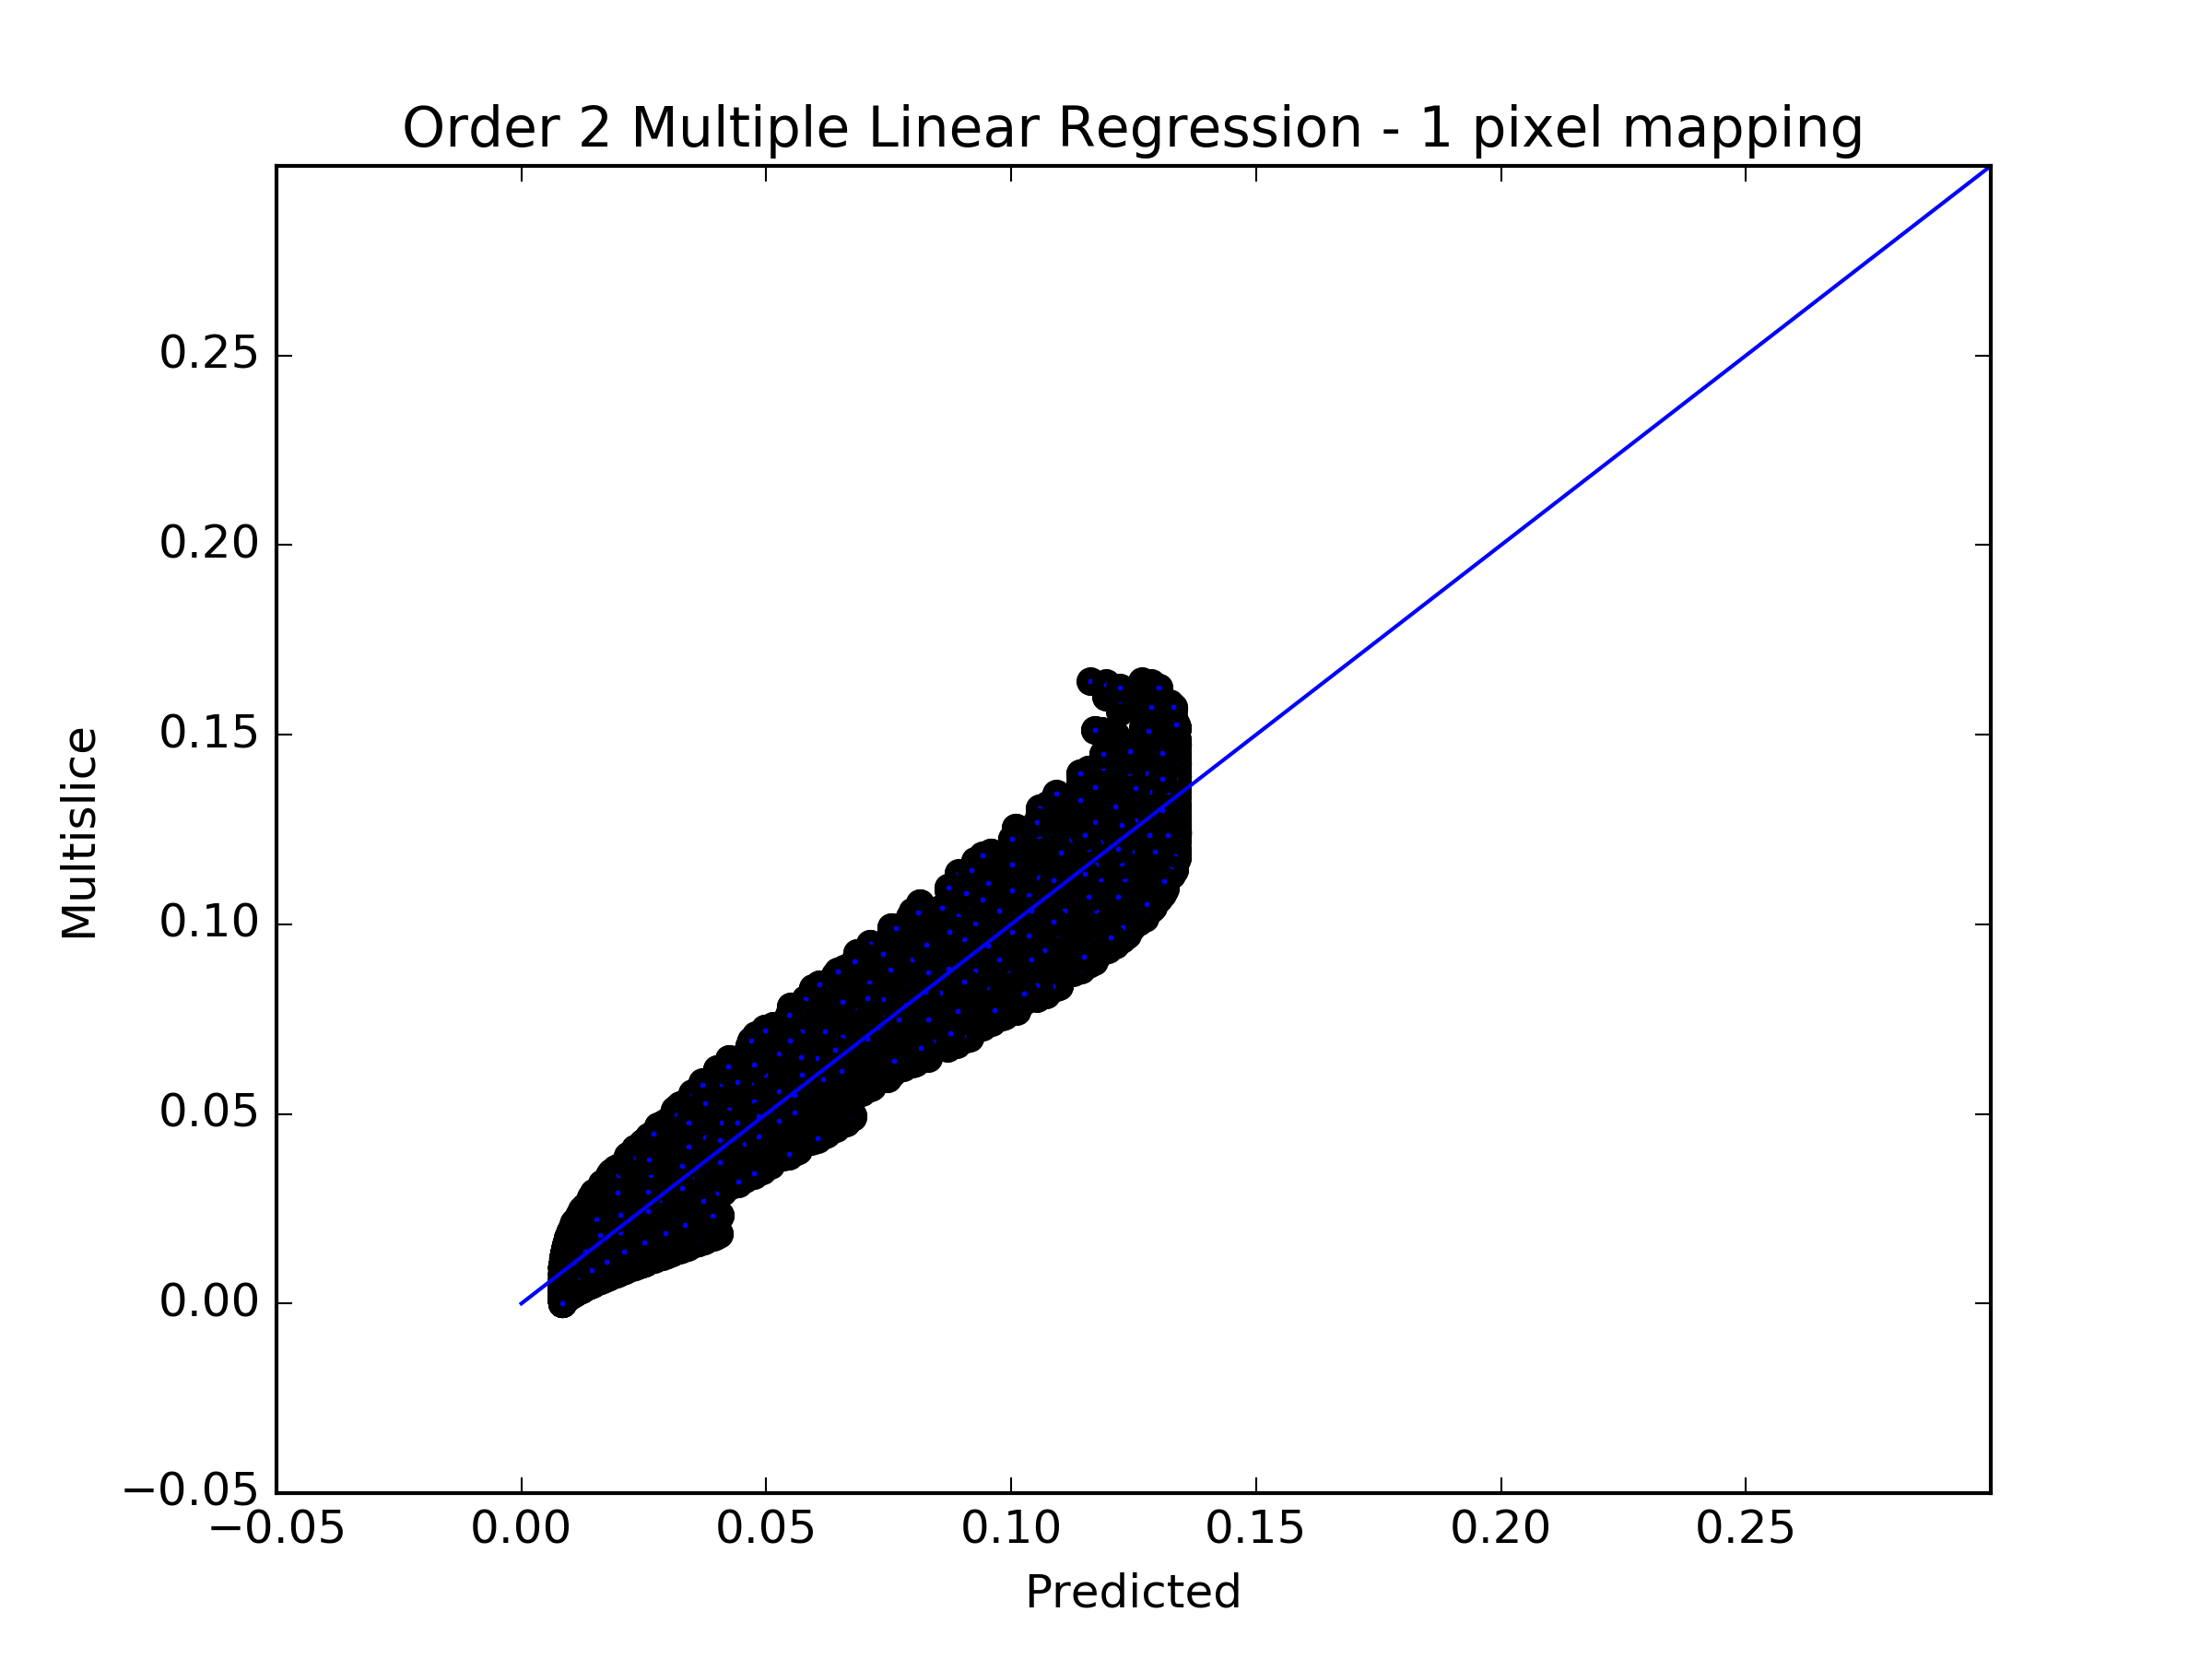
\includegraphics[width=.9\linewidth]{./images/olr_order2_1pixel.png}\\
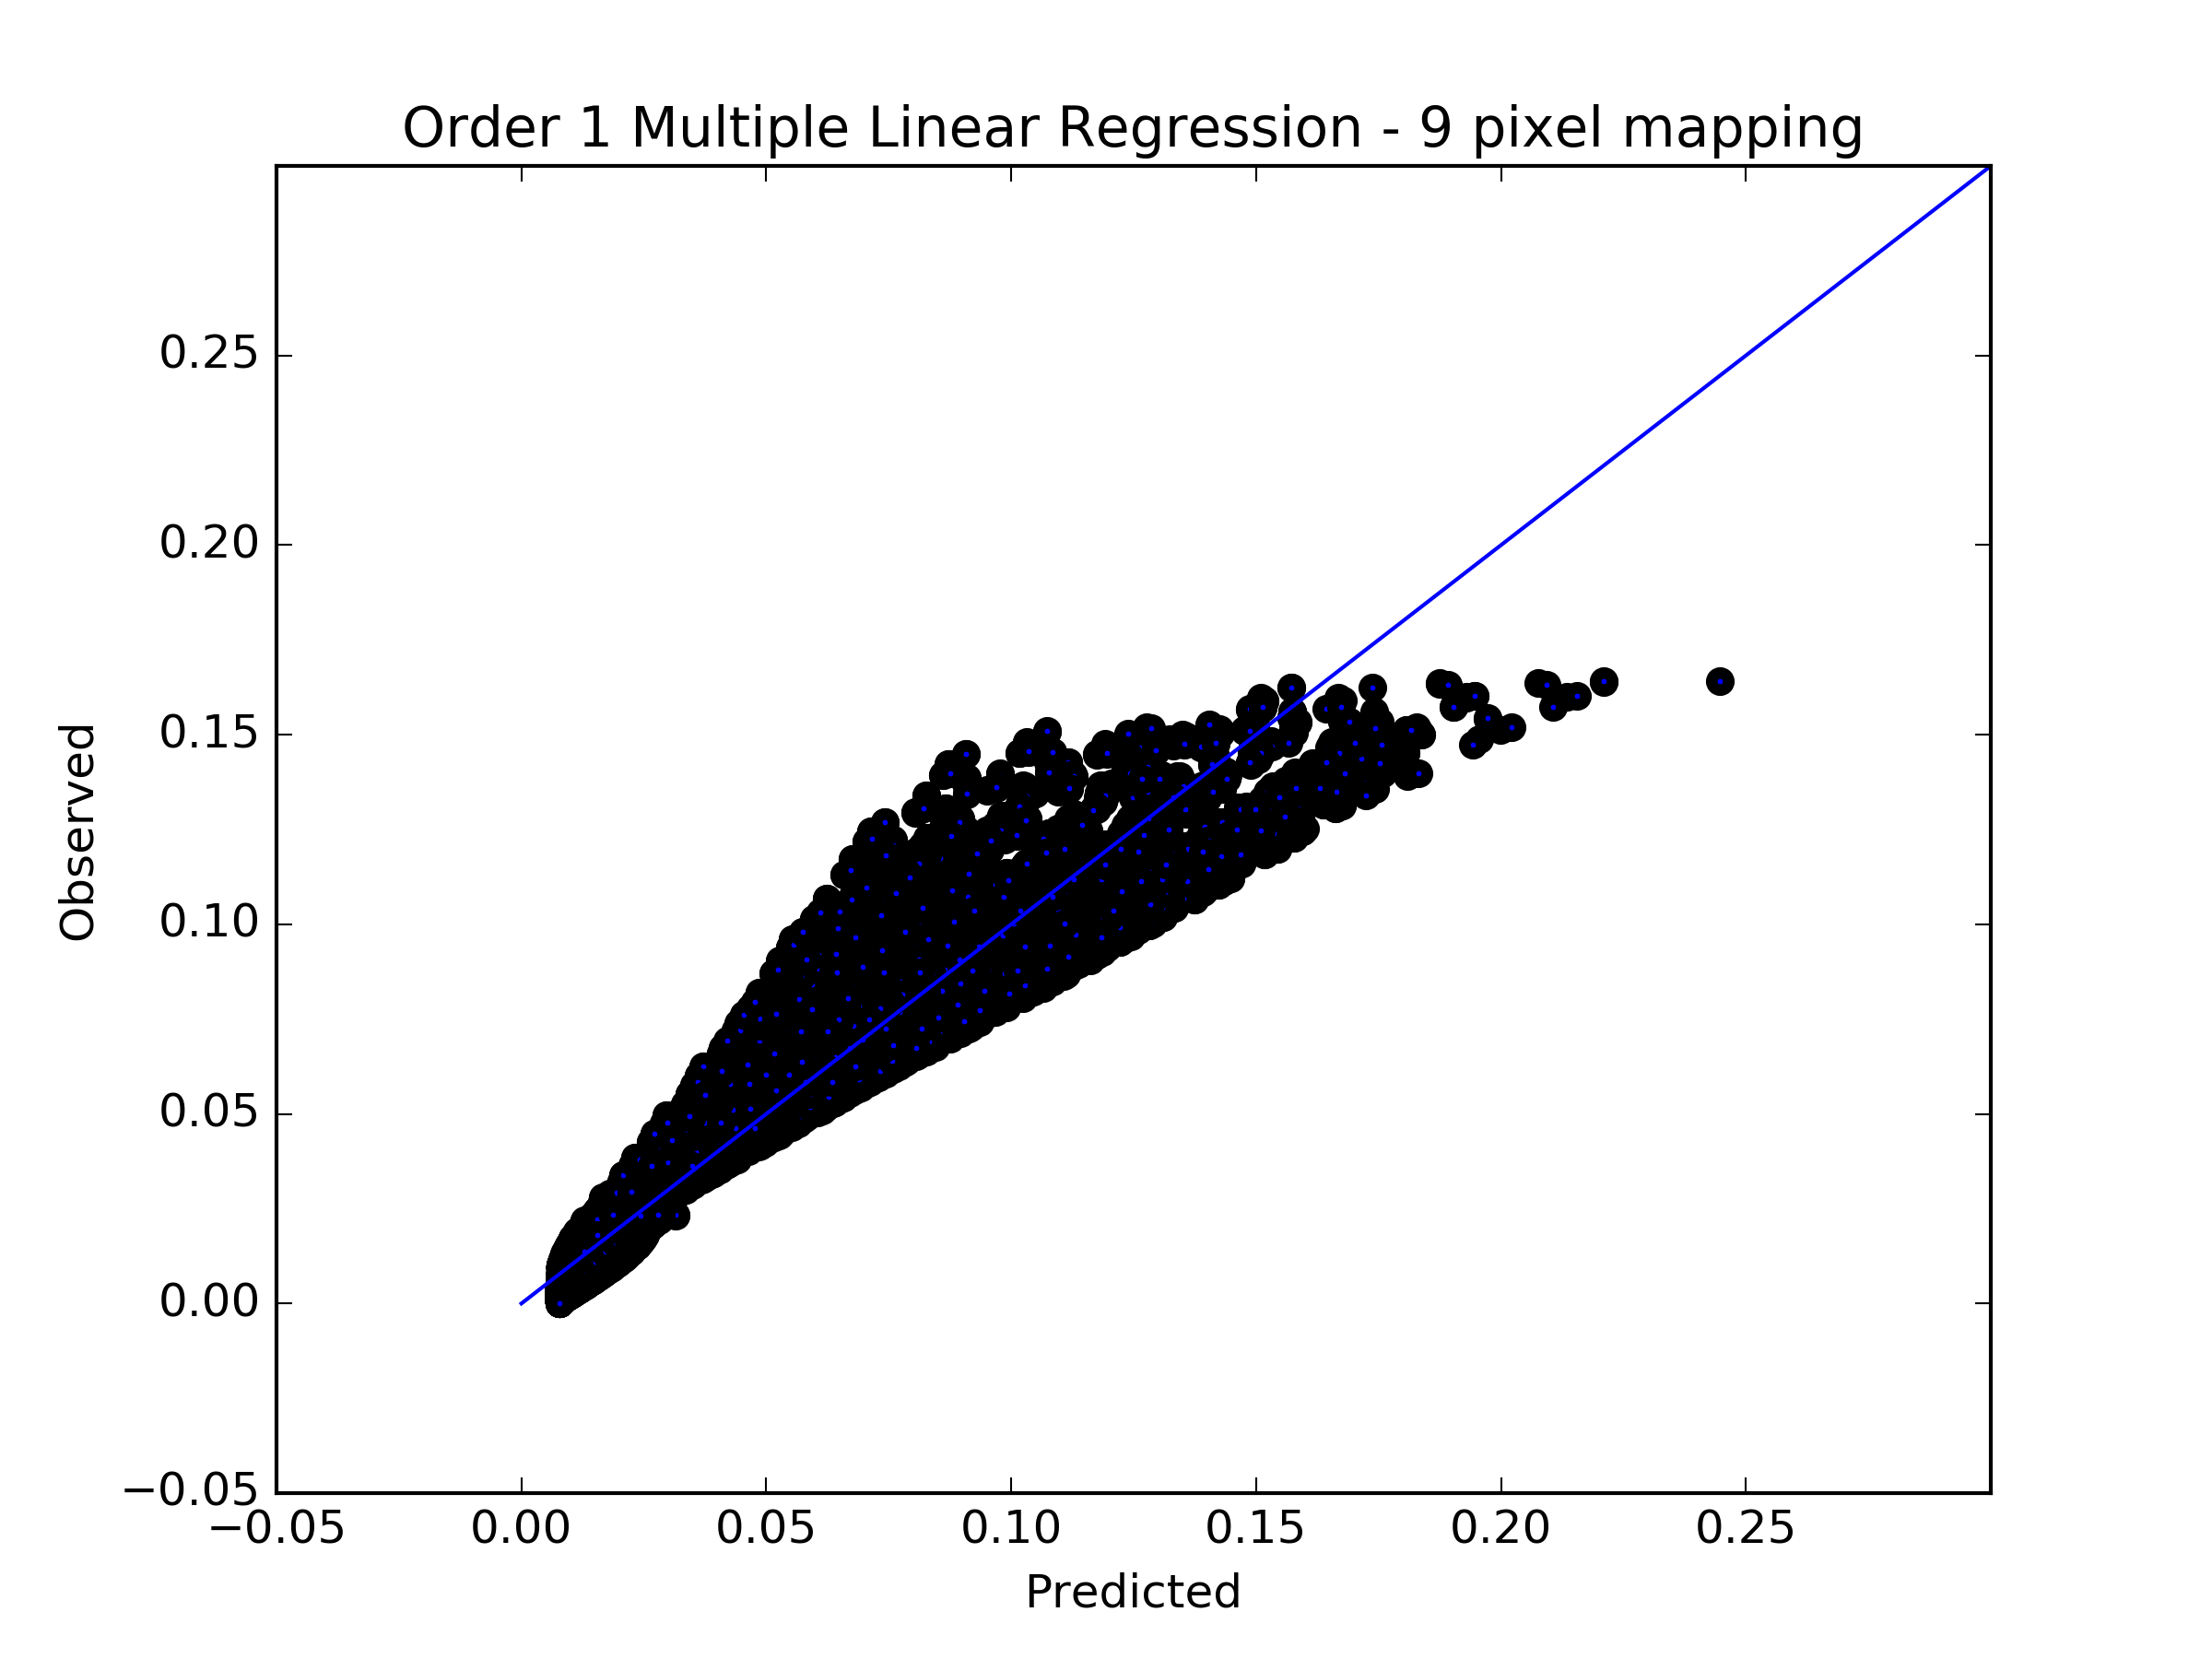
\includegraphics[width=.9\linewidth]{./images/olr_order1_9pixel.png}\\
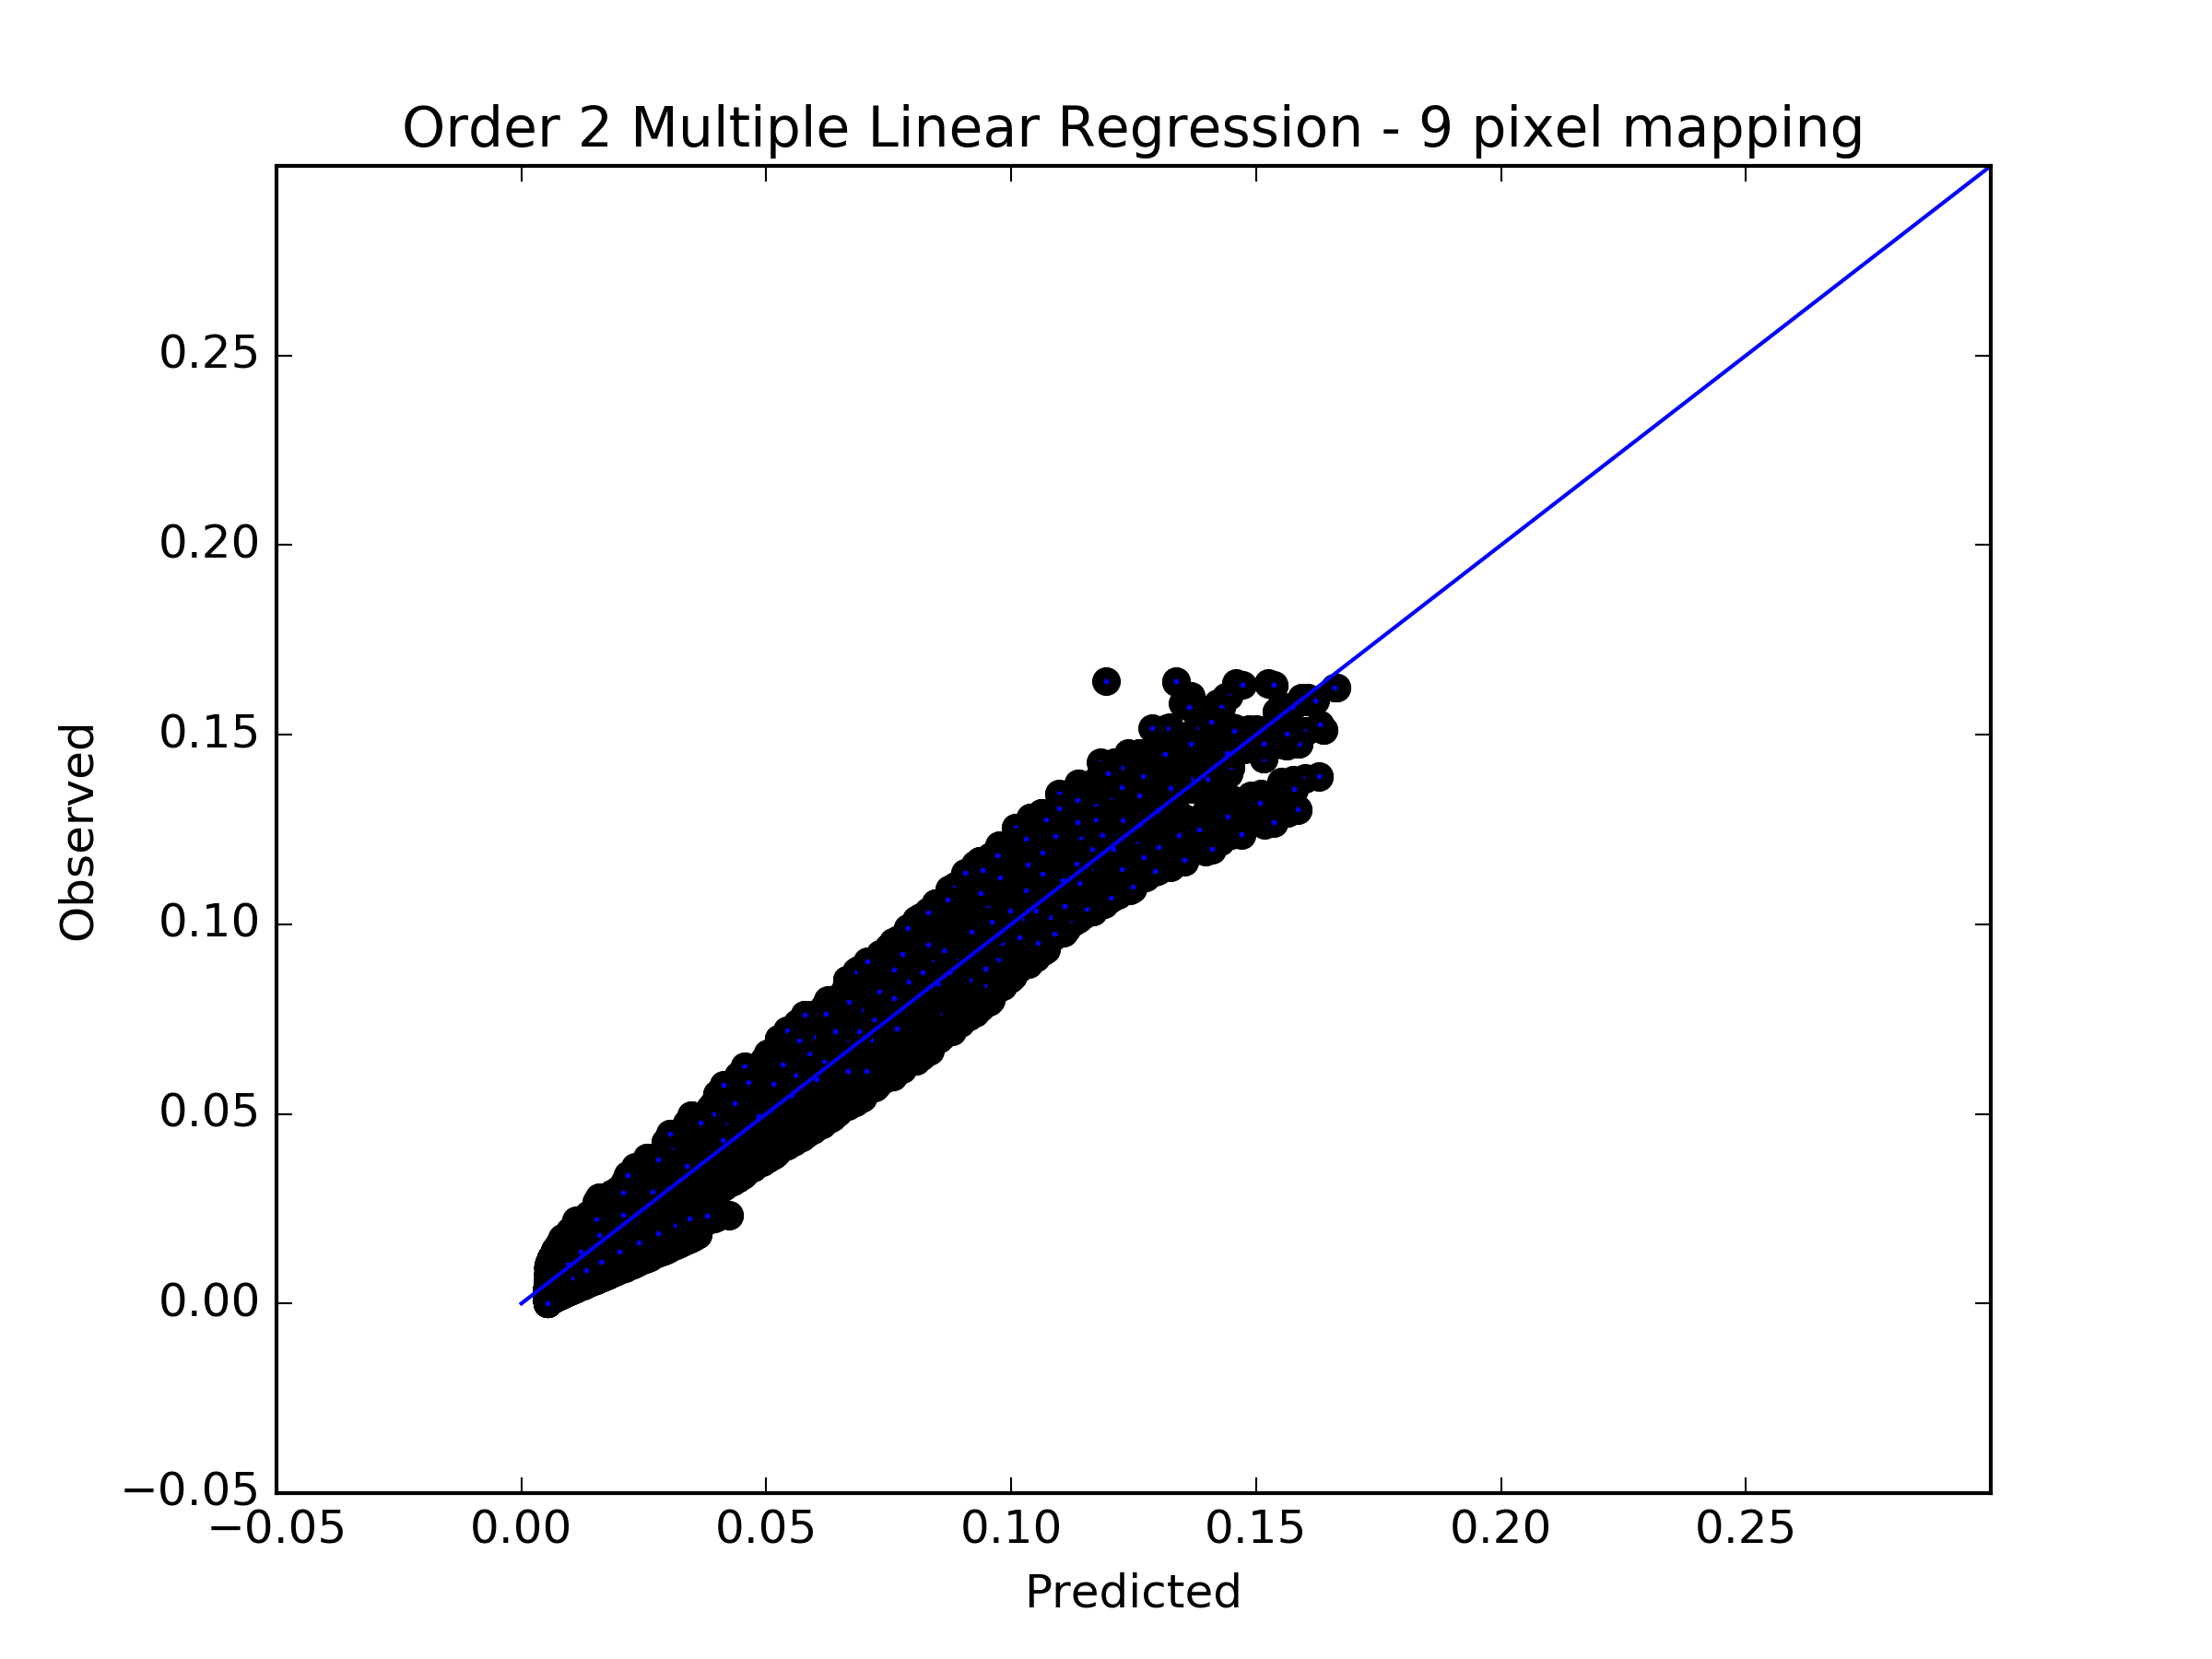
\includegraphics[width=.9\linewidth]{./images/olr_order2_9pixel.png}\\
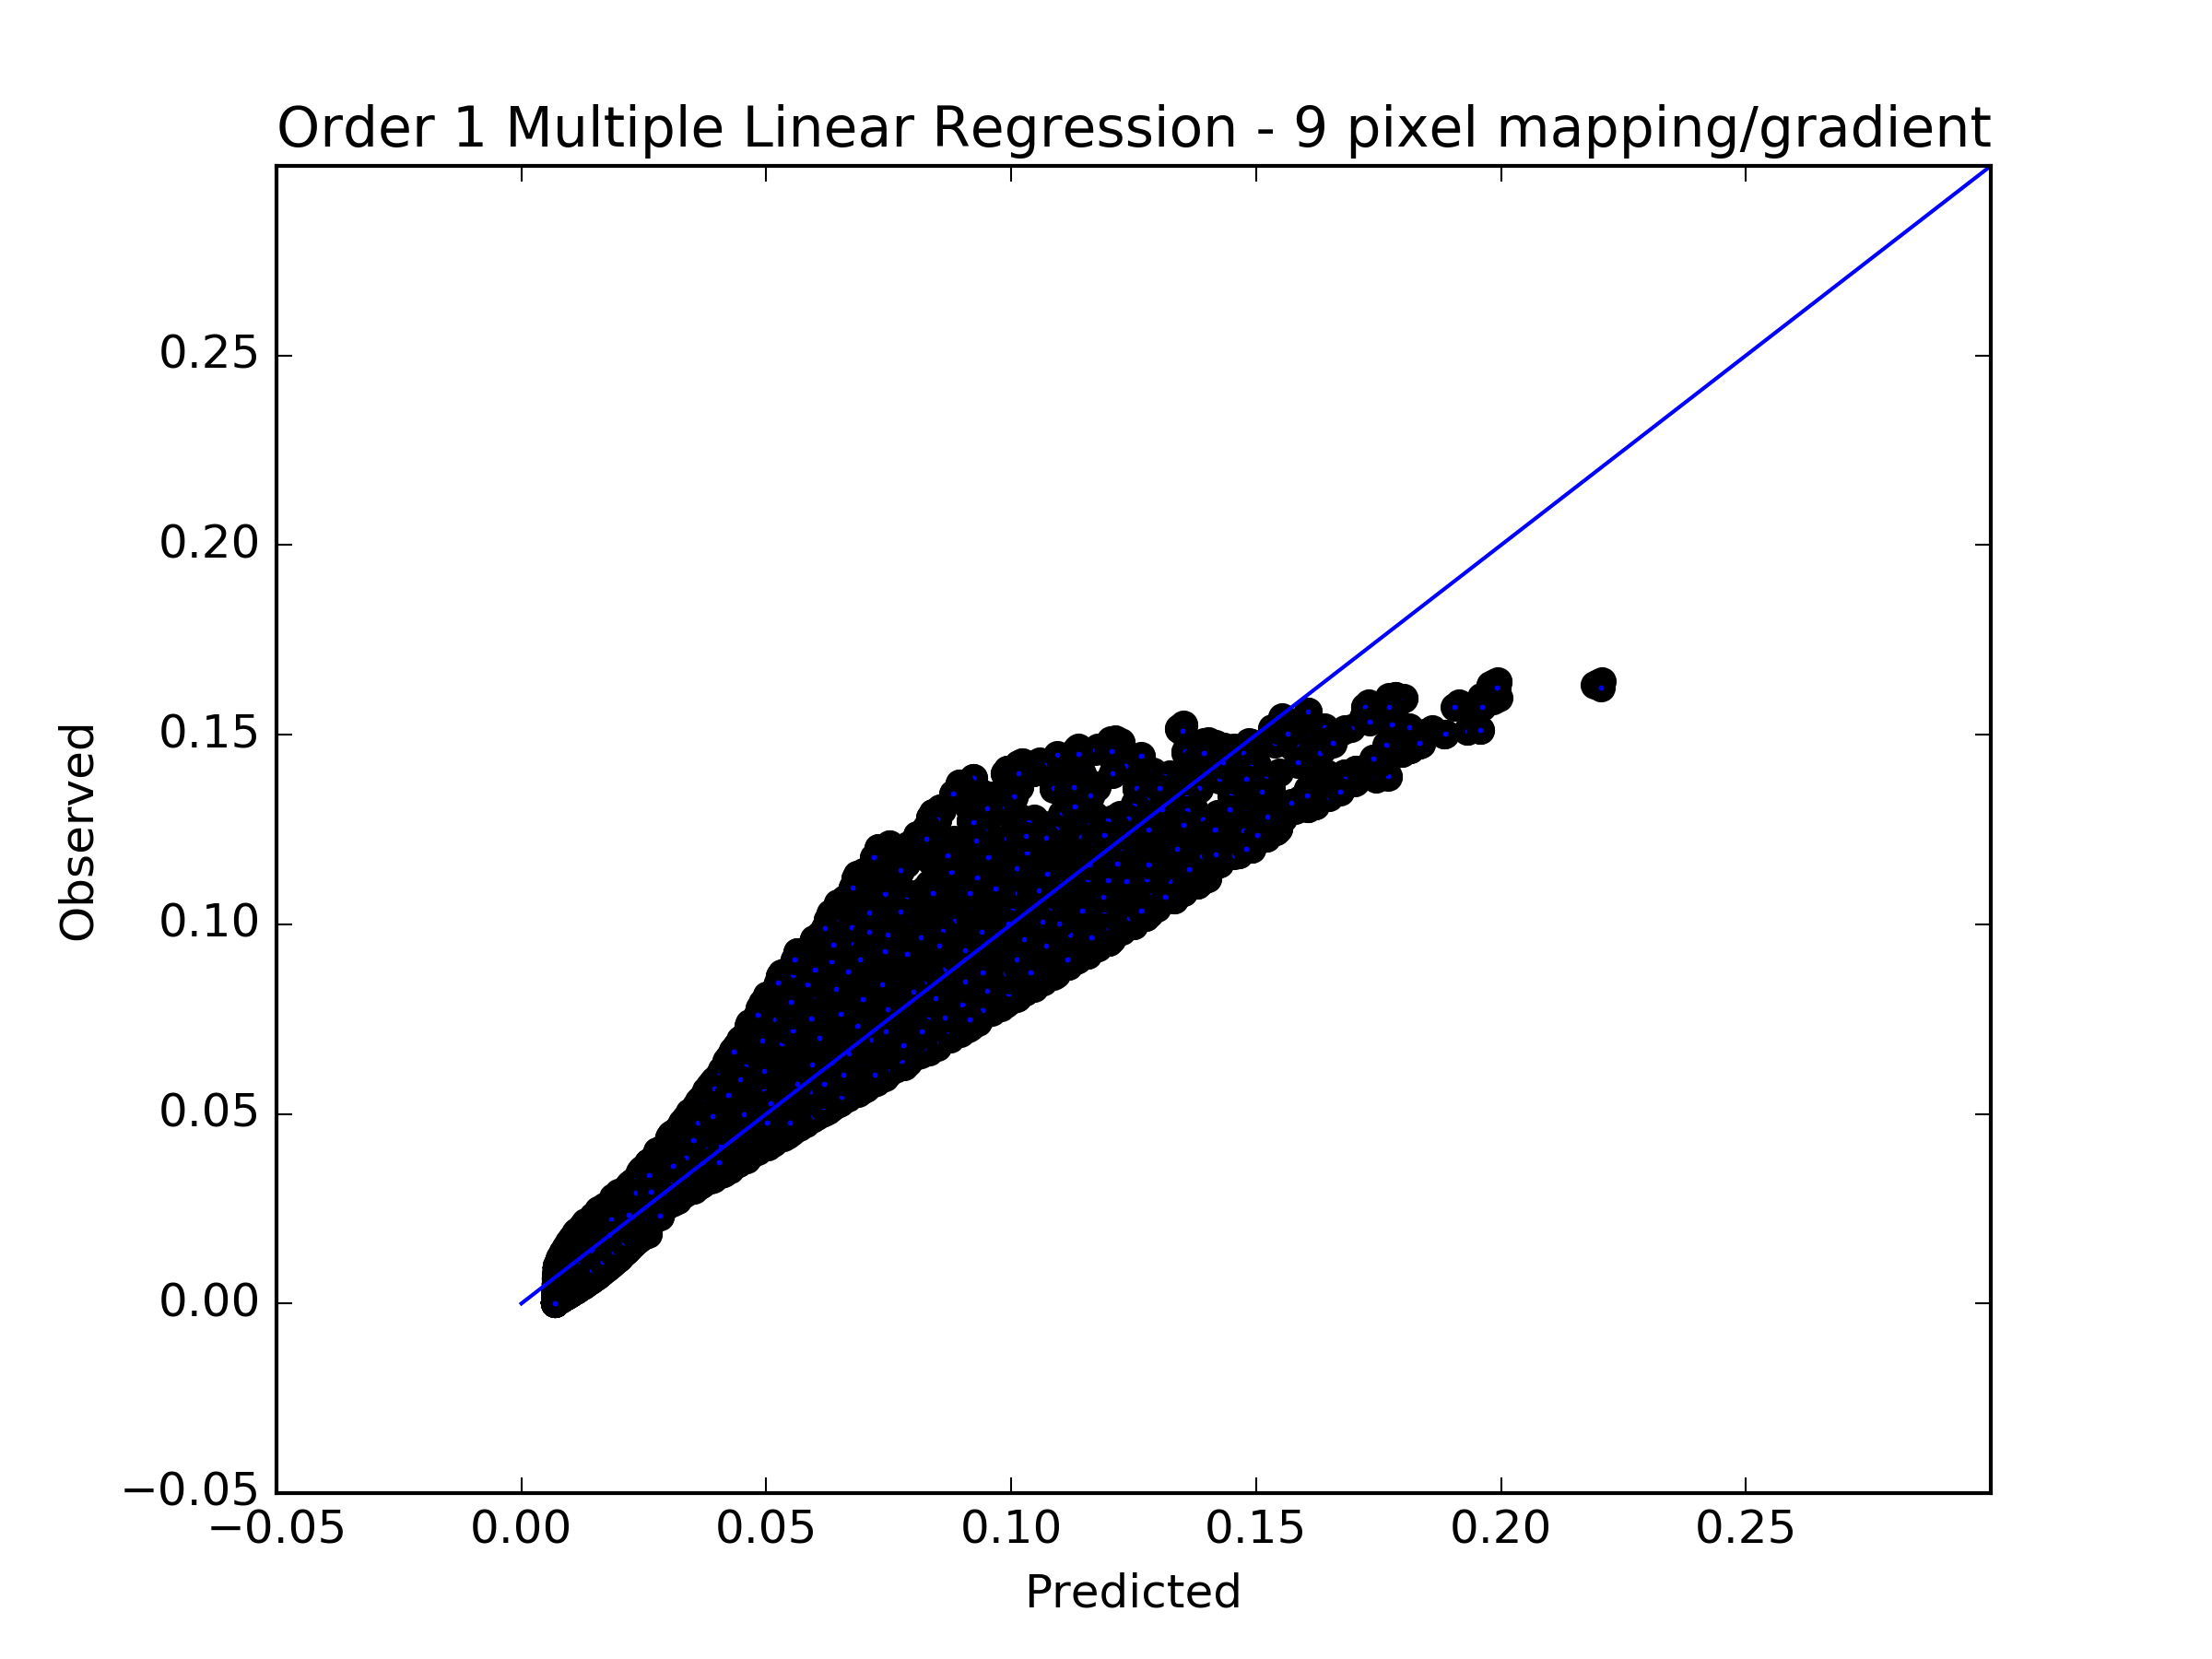
\includegraphics[width=.9\linewidth]{./images/olr_order1_9pixel_grad.png}\\
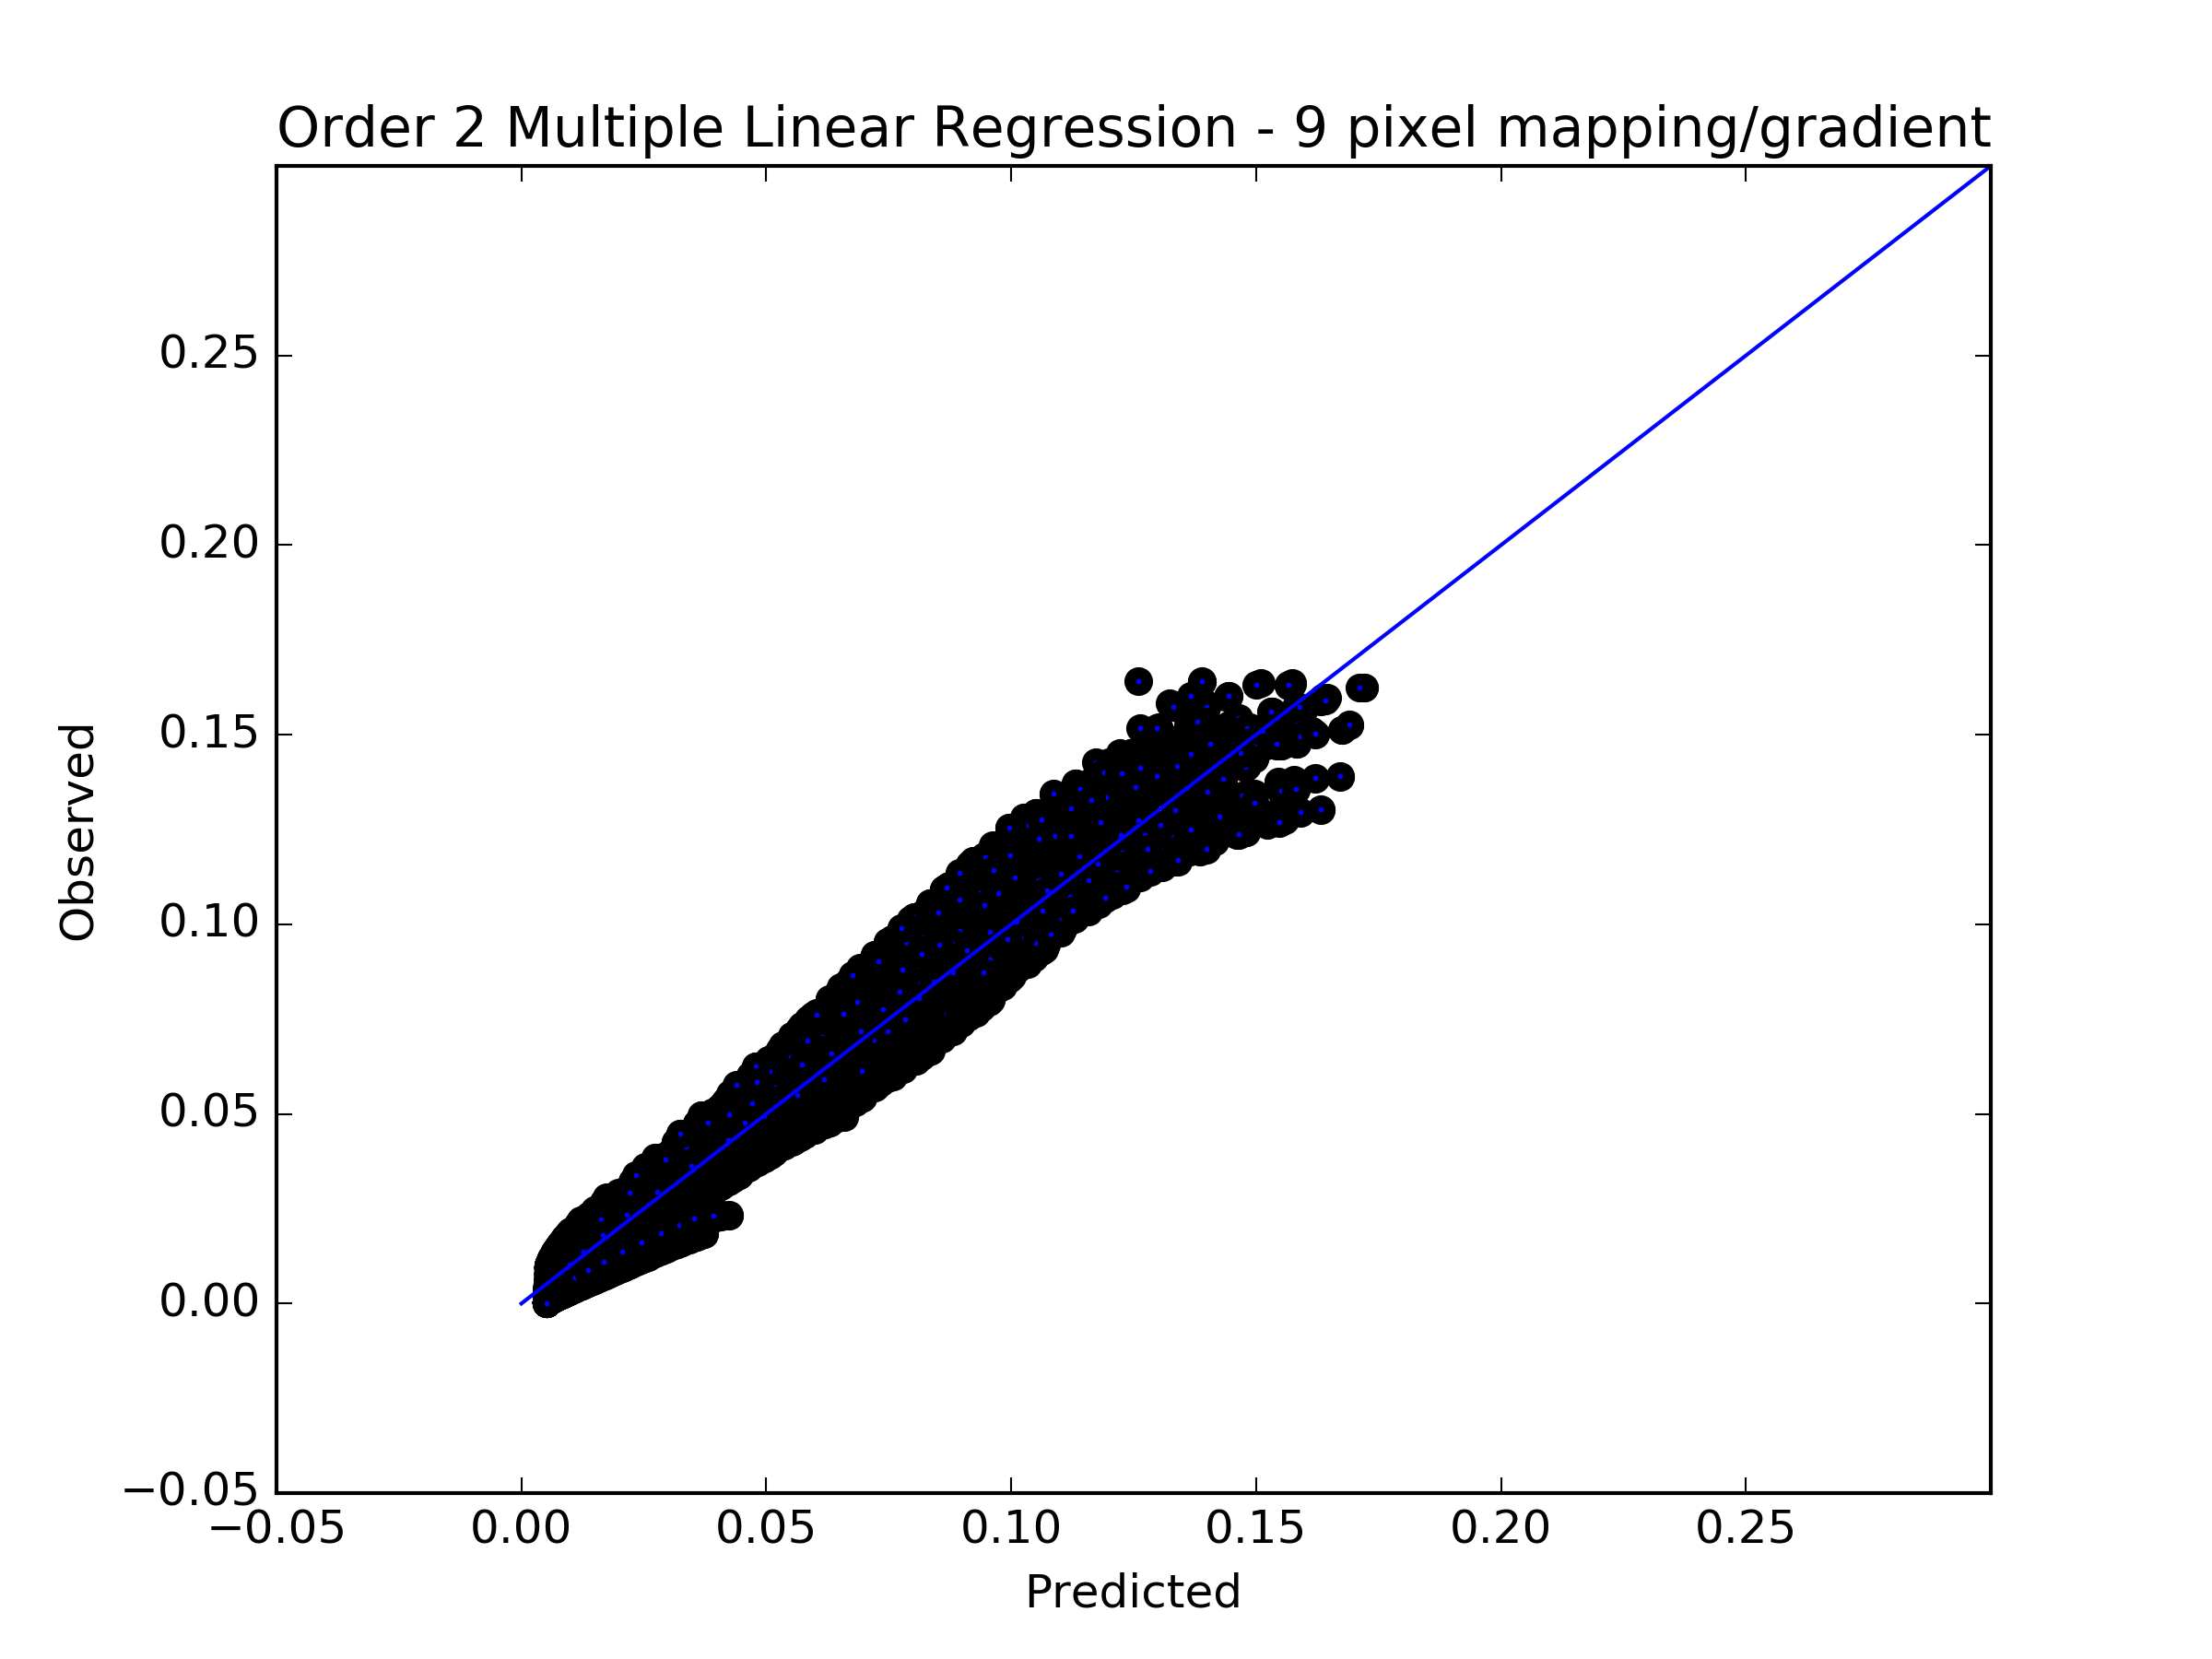
\includegraphics[width=.9\linewidth]{./images/olr_order2_9pixel_grad.png}\\

\begin{itemize}
\item Python files: olr2.py
\end{itemize}
\pagebreak
\section{Data}
\label{sec-2}
\subsubsection{Convolution}
\label{sec-2-0-1}
\begin{itemize}
\item 50 by 36 by 20
\item intensities = [0, 139.7768]
\end{itemize}

\subsubsection{Multislice}
\label{sec-2-0-2}
\begin{itemize}
\item 50 by 36 by 20
\item intensities = [0, 0.1641]
\end{itemize}
% Emacs 24.5.1 (Org mode 8.2.10)
\end{document}
